\subsection{Request Approval}

\begin{figure}[H]
    \centering
    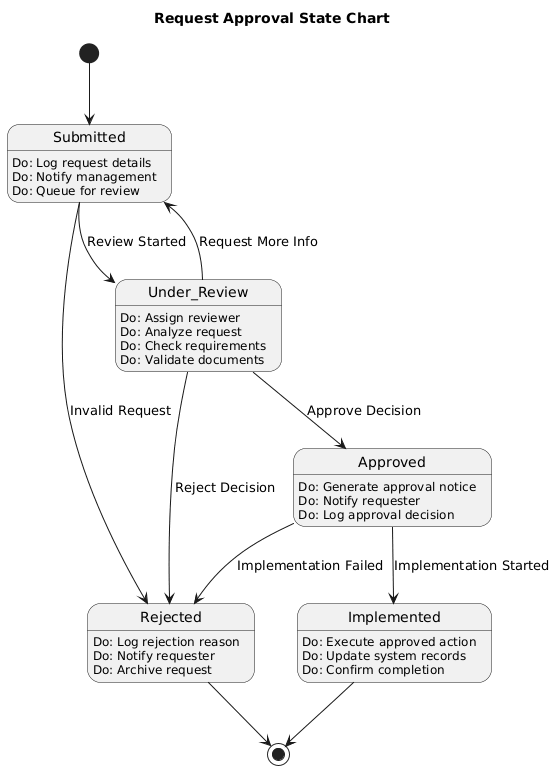
\includegraphics[width=0.8\textwidth]{graphics/chapter5/request.png}
    \caption{Request Approval}
    \label{fig:Request_Approval}
\end{figure}

\newpage

\noindent \textbf{Description}
\begin{itemize}
  \item \textbf{Purpose:} Model the lifecycle of approval requests from submission to final implementation or rejection.
  
  \item \textbf{States:} 
    \textit{Submitted} (Do: Log request details, Notify management, Queue for review);
    \textit{Under Review} (Do: Assign reviewer, Analyze request, Check requirements, Validate documents);
    \textit{Approved} (Do: Generate approval notice, Notify requester, Log approval decision);
    \textit{Rejected} (Do: Log rejection reason, Notify requester, Archive request);
    \textit{Implemented} (Do: Execute approved action, Update system records, Confirm completion).
  
  \item \textbf{Transitions:}
    Request Submission $\Rightarrow$ \textit{Submitted};
    Review Started $\Rightarrow$ \textit{Under Review};
    Approve Decision $\Rightarrow$ \textit{Approved};
    Reject Decision $\Rightarrow$ \textit{Rejected};
    Invalid Request from \textit{Submitted} $\Rightarrow$ \textit{Rejected};
    Request More Info from \textit{Under Review} $\Rightarrow$ \textit{Submitted};
    Implementation Started $\Rightarrow$ \textit{Implemented};
    Implementation Failed from \textit{Approved} $\Rightarrow$ \textit{Rejected}.
  
  \item \textbf{Start/End:} 
    Initial node $\rightarrow$ \textit{Submitted}; 
    \textit{Implemented} $\rightarrow$ final node;
    \textit{Rejected} $\rightarrow$ final node.
  
  \item \textbf{Notes:} 
    Only \textit{Under Review} requests are actively being processed by management; 
    \textit{Submitted} requests wait in queue for reviewer assignment;
    \textit{Rejected} requests can be resubmitted as new requests if corrected;
    \textit{Approved} requests must be implemented to complete the process;
    System tracks review time and automatically escalates overdue requests;
    Both \textit{Implemented} and \textit{Rejected} are terminal states in this chart.
\end{itemize}
